\documentclass{article}
\usepackage{times}
\usepackage{graphicx}
\usepackage{subfigure} 
\usepackage{natbib}
\usepackage{algorithm}
\usepackage{algorithmic}
\usepackage{subfigure}
\usepackage{hyperref}
\newcommand{\theHalgorithm}{\arabic{algorithm}} % Fixes misbehavior of conflicting packages.
\usepackage{icml2016/icml2016} 

\icmltitlerunning{Approximate State Abstraction}

% --- Note Commands ---
\usepackage{color}
\newcommand\dnote[1]{\textcolor{blue}{Dave: #1}}
\newcommand\enote[1]{\textcolor{green}{Ellis: #1}}

% --- DOCUMENT ---
\begin{document}

\twocolumn[
\icmltitle{Approximate State Abstraction}

% Paper Meta Info
\icmlauthor{David Abel}{david_abel@brown.edu}
\icmladdress{Brown University,
            115 Waterman Street, Providence, RI 02906}
\icmlauthor{D. Ellis Hershkowitz}{david_hershkowitz@brown.edu}
\icmladdress{Brown University,
            115 Waterman Street, Providence, RI 02906}
\icmlauthor{Michael L.\ Littman}{michael_littman@brown.edu}
\icmladdress{Brown University,
            115 Waterman Street, Providence, RI 02906}
    
\icmlkeywords{Reinforcement Learning, State Aggregation, State Abstraction, Planning, MDP}
            
\vskip 0.3in
]


% --- ABSTRACT ---
\begin{abstract}
The combinatorial explosion that plagues planning and reinforcement-learning algorithms can be reversed using abstraction. For instance, prohibitively difficult task representations can be condensed so that solutions are tractably computable. In this work, we investigate a theoretical framework for approximate state abstraction that preserves near optimal behavior. Reinforcement learning agents using these abstractions may treat experiences that resemble each other as equivalent, and generalize knowledge to novel scenarios based on prior experiences. We present theoretical guarantees of the quality of value functions derived from three classes of approximate state abstraction. Additionally, we empirically evaluate the relationship between the degree of approximation and the degree of abstraction achieved, as well as the tradeoff between approximation magnitude and optimality of behavior.
\end{abstract}

% Set of actions within epsilon (Q*) is the same for two states? Better than boltzmann.


% --- SECTION: Introduction ---
\section{Introduction}

\begin{itemize}
\item Solving MDPs is P-Complete, where the dominant factor is $|\mathcal{S}|$.
\item Sample complexity is {\it also} dominated by $|\mathcal{S}|$.
\item To make MDPs with large $|\mathcal{S}|$ tractable, we can reduce the MDPs to a simpler form.
\item In this work, we show that compressing MDPs in a particular way allows for the transfer of bounded-error solutions between the compressed MDP and ground MDP.
\item Q: Why approximate?
\item A: Approximate can compress strictly more than compression based on equality
\item A: Approximate compression requires the type of knowledge that we could imagine learning (i.e.. approximate knowledge)
\end{itemize}


% --- SECTION: Related Work ---
\section{Related Work}

% Lihong/Walsh/Littman: Towards a unified theory...
Citation test~\cite{li2006towards}

% Nan/Lihong

% Approximate bisimulation

% David Silver: Options/State Abstraction?

% Russell? PHAM/HAM/ALisp

% Konidaris? Options induce symbolic representation on continuous state space

% Littman: Relocatable Action Models

% Stone: State Abstraction Discovery from Irrelevant State Vars

% Others...


% --- SECTION: Background ---
\section{Background}

% Quick MDP blurb?

% Phi notation

% Evluation of Abstract MDP

% Abstract MDP, Ground MDP, Homogenizing Gun

% Previous state aggregation stuff? Or should be in related work?


% --- SECTION: State Abstraction ---
\section{Approximate State Abstraction}

% Explain each of the Phis

% One theorem, each separate phi is its own lemma.


% Subsections for proofs for each phi
\dnote{Insert lemma for each phi as their subsection}

% Subsection: 

% Subsection: Phi_M
\subsection{$\Phi_M$}


% Subsection: Phi_Q
\subsection{$\Phi_Q^*$}


% Subsection: Phi_D
\subsection{$\Phi_D$}



% Subsection: Phi_B
\subsection{$\Phi_B$}
\dnote{$\Phi_{Boltzmann}$}


% Subsection: Other Abstractions
\subsection{Other Abstractions}

% Discussion of other abstractions we looked into

% Some abstractions DON'T preserve a meaningful notion of optimality.



% --- SECTION: Example Domains ---
\section{Example Domains}

\dnote{For each section, we'll include a plot comparing $\epsilon$ to \# states, and $\epsilon$ to performance. For UpWorld and NChain, we can include visuals of uncompressed and compressed (not useful for trench).}

% Subsection: UpWorld
\subsection{UpWorld}

\dnote{As part of UpWorld we can include the result about the unbounded improvement in sample complexity (small lemma or something?)}

% Insert visual and/or stats on number of states and performance of VI solving the abstract MDP and evaluating the resulting policy on the original MDP


% Subsection: NChain
\subsection{NChain}

% Insert visual and/or stats on number of states and performance of VI solving the abstract MDP and evaluating the resulting policy on the original MDP


% Subsection: Trench
\subsection{Trench}

% Insert visual and/or stats on number of states and performance of VI solving the abstract MDP and evaluating the resulting policy on the original MDP


% Figure: The Trench Problem
\begin{figure}[h]
\centering
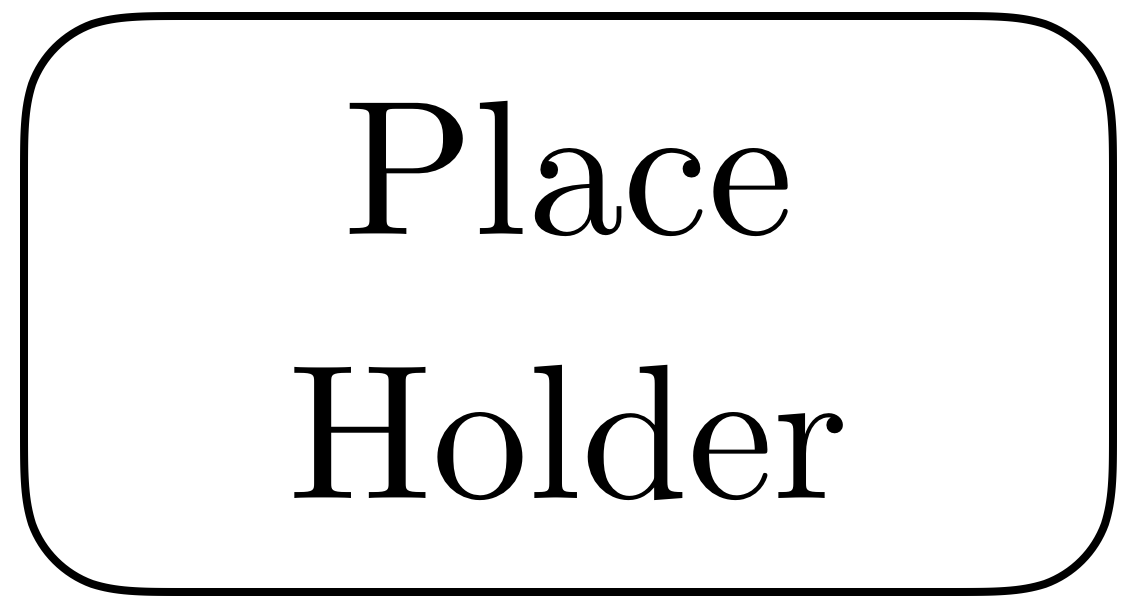
\includegraphics[width=0.42\columnwidth]{figures/placeholder.png}
\caption{The Trench Problem}
\label{fig:trench}
\end{figure}


% --- SECTION: Approximate Abstraction on Example Domains ---
\section{Approximate Abstraction on Example Domains}

% Figure: Epsilon vs. #States for all three sample domains.
\begin{figure}
\subfigure[UpWorld]{
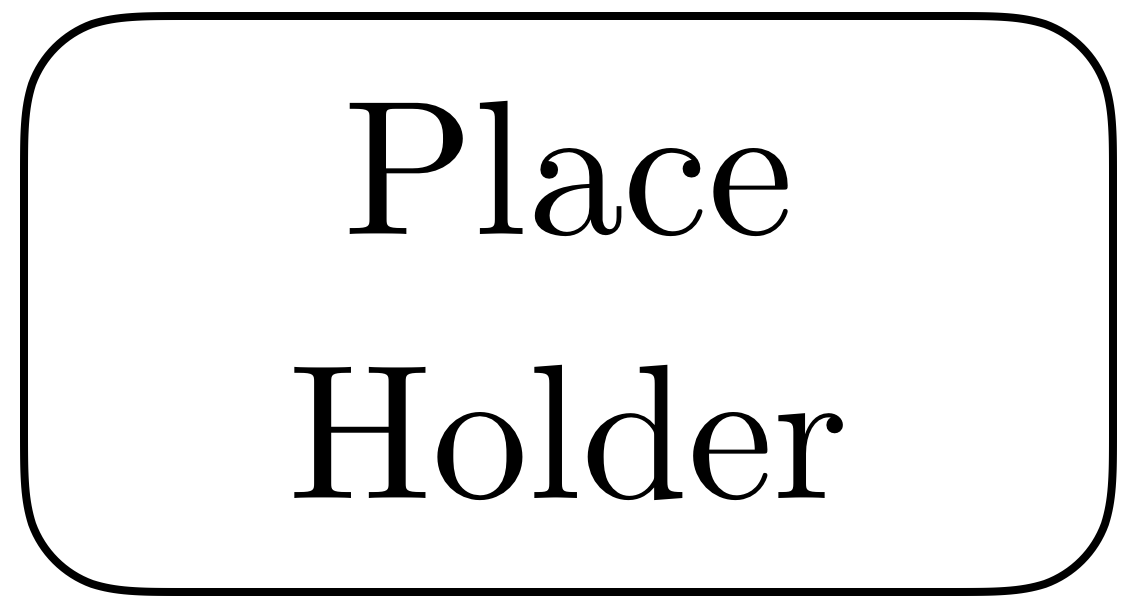
\includegraphics[width=0.28\columnwidth]{figures/placeholder.png}}
\subfigure[NChain]{
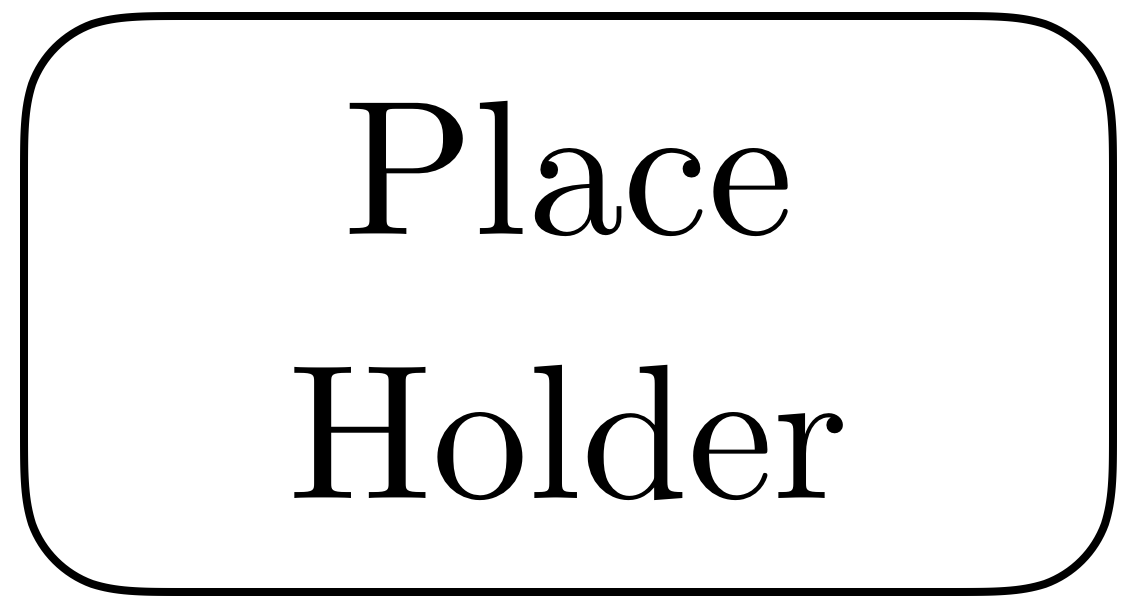
\includegraphics[width=0.28\columnwidth]{figures/placeholder.png}}
\subfigure[Trench]{
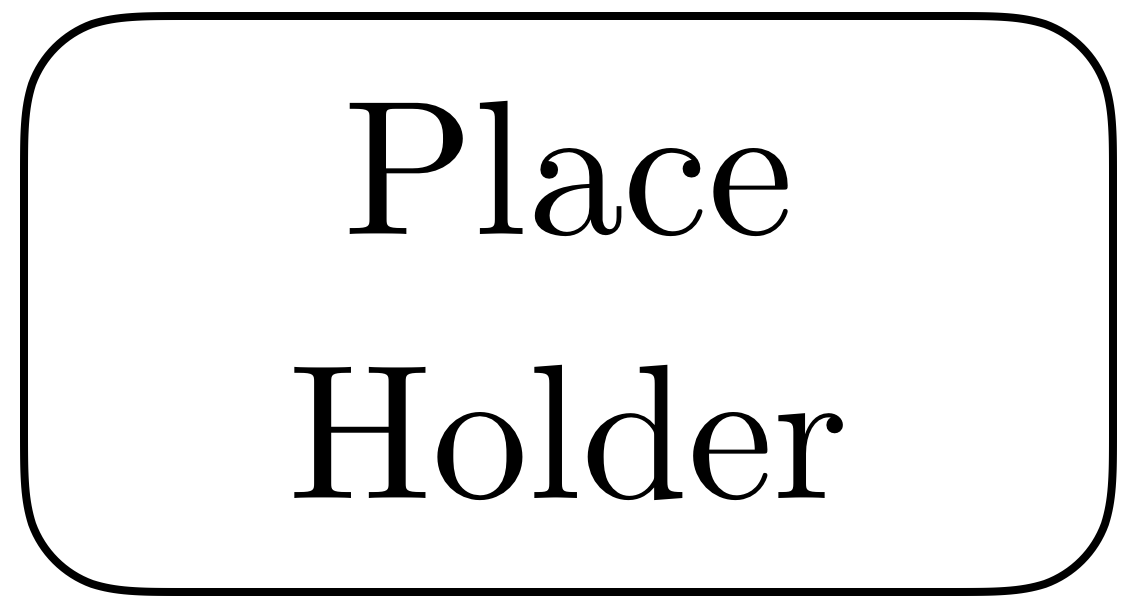
\includegraphics[width=0.28\columnwidth]{figures/placeholder.png}}
\label{fig:eps-states}
\caption{$\epsilon$ vs. Num States}
\end{figure} 

% Figure: Epsilon vs. Error in Abstract Value Function
\begin{figure}
\subfigure[UpWorld]{
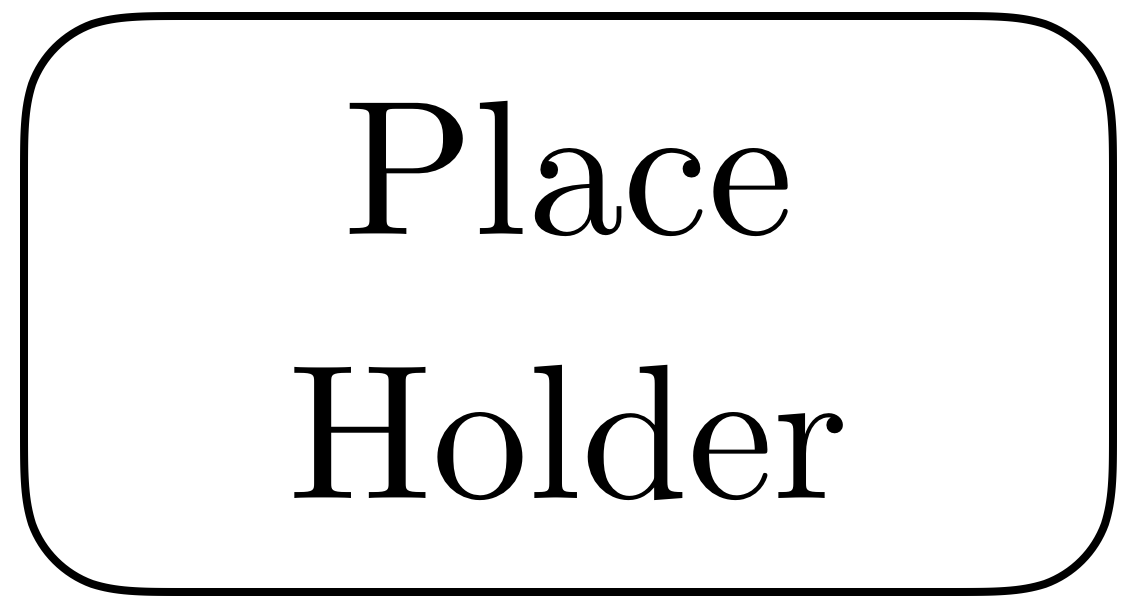
\includegraphics[width=0.28\columnwidth]{figures/placeholder.png}}
\subfigure[NChain]{
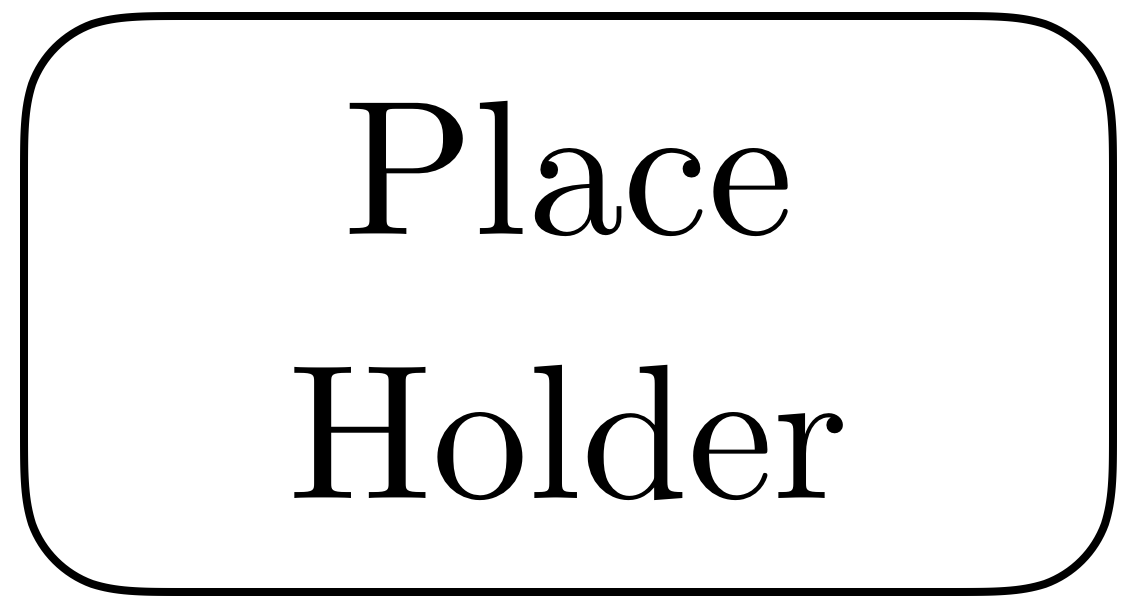
\includegraphics[width=0.28\columnwidth]{figures/placeholder.png}}
\subfigure[Trench]{
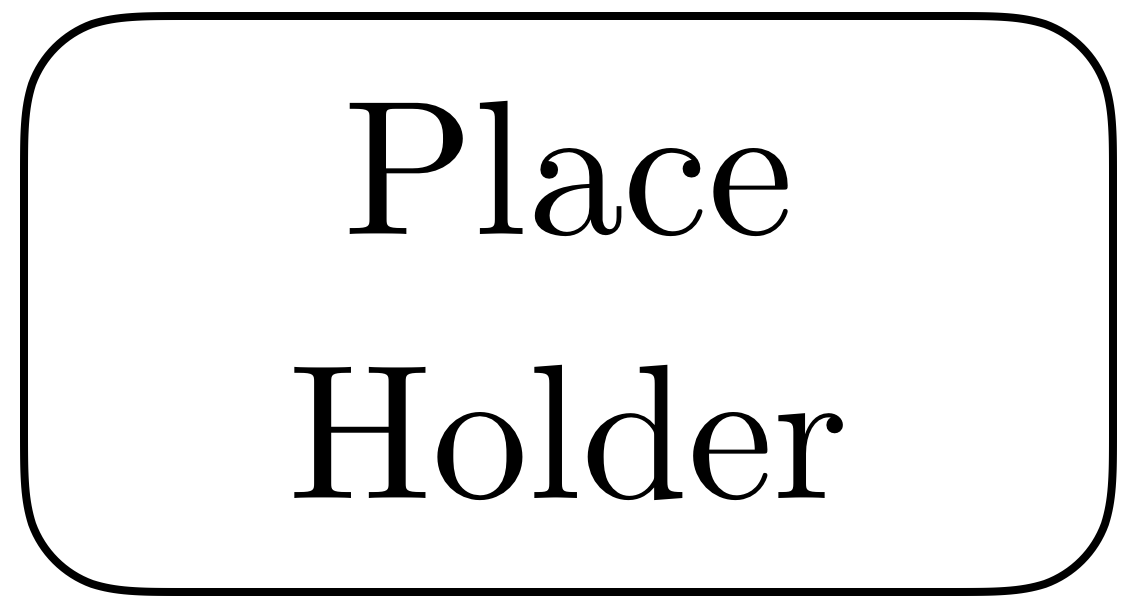
\includegraphics[width=0.28\columnwidth]{figures/placeholder.png}}
\label{fig:eps-states}
\caption{$\epsilon$ vs. Error in Abstract Value Function}
\end{figure} 



% Subsection: Abstract Domain Visualizations
\subsection{Abstract Domain Visualizations}

% Figure: UpWorld MDP visuals
\begin{figure}[h]
\centering
\subfigure[UpWorld]{
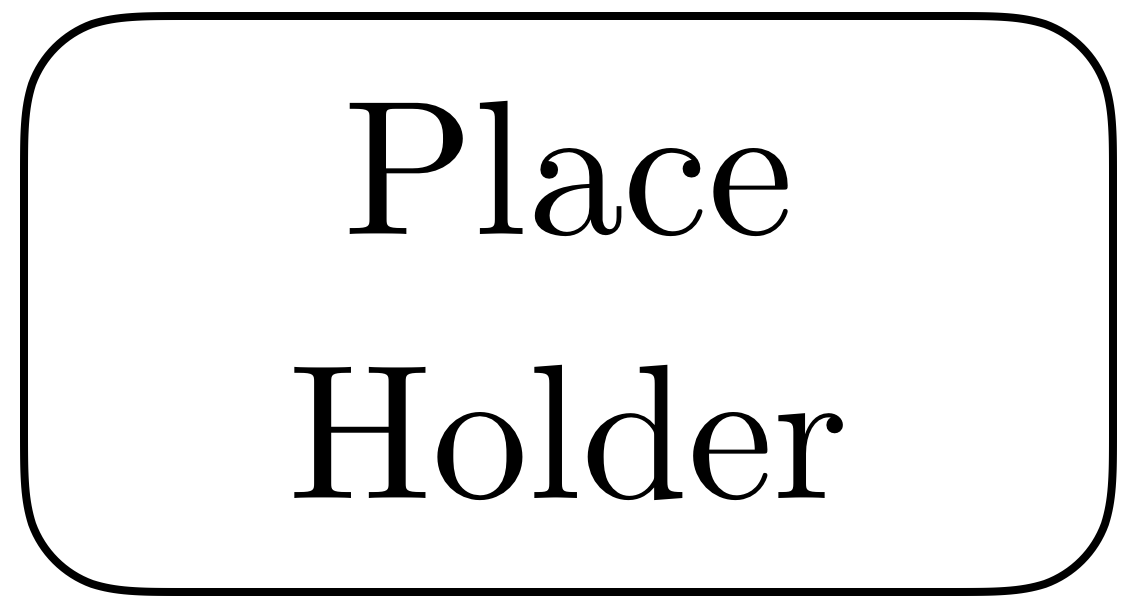
\includegraphics[width=0.46\columnwidth]{figures/placeholder.png}}
\hspace{3mm}
\subfigure[Abstracted UpWorld]{
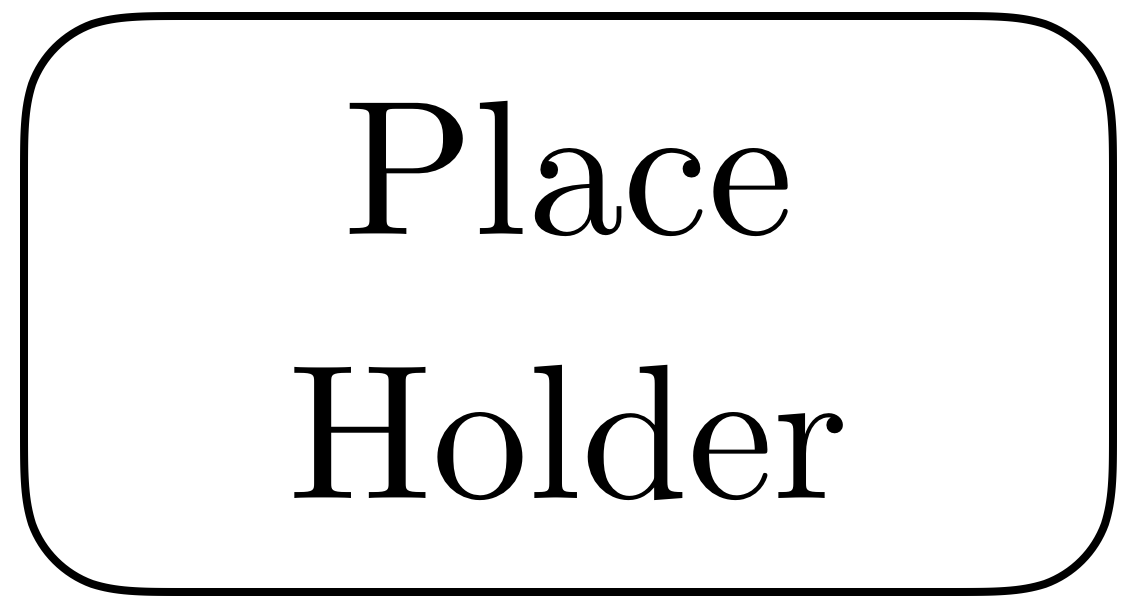
\includegraphics[width=0.46\columnwidth]{figures/placeholder.png}}
\caption{Visualization of Original UpWorld vs. Abstracted UpWorld}
\end{figure}

% Figure: NChain MDP visuals
\begin{figure}[h]
\centering
\subfigure[NChain]{
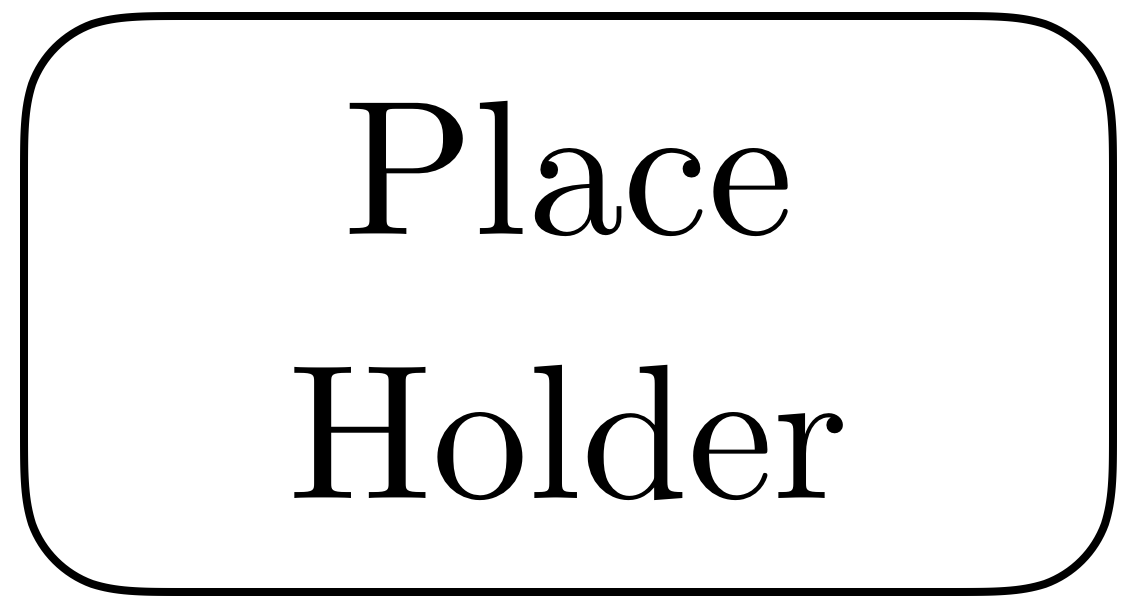
\includegraphics[width=0.46\columnwidth]{figures/placeholder.png}}
\hspace{3mm}
\subfigure[Abstracted NChain ]{
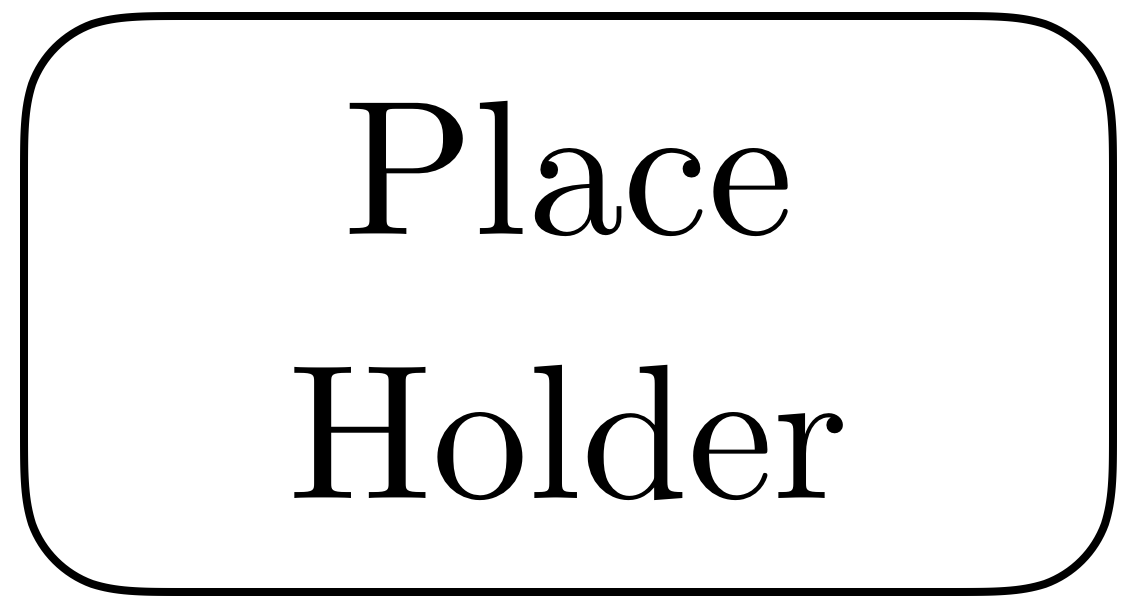
\includegraphics[width=0.46\columnwidth]{figures/placeholder.png}}
\caption{Visualization of Original NChain vs. Abstracted NChain}
\end{figure}






% --- SECTION: Conclusion ---
\section{Conclusion}

% Summary

% Future Work
\begin{enumerate}
\item Learning Phi
\begin{itemize}
\item Exploration vs. Exploitation problem is different while trying to learn Phi
\end{itemize}
\item Compressibility
\begin{itemize}
\item Relationship between approximate abstract and compressibility
\end{itemize}
\item POMDP and abstraction
\end{enumerate}





% --- BIBLIOGRAPHY ---
\bibliographystyle{icml2016/icml2016}
\bibliography{state_abs}

\end{document}
